
\documentclass[12pt,a4paper]{scrartcl}

\usepackage[a4paper, left=2cm, right=1cm, bottom=1cm, top=1cm, includeheadfoot]{geometry}
\usepackage[ngerman]{babel}
\usepackage[utf8]{inputenc} % comment this if you uncomment utf8x
%\usepackage[utf8x]{inputenc} % uncomment this if there are problems with 'ä', 'ü', 'ö'
\usepackage{ucs}
\usepackage[usenames,dvipsnames]{xcolor}
\usepackage[fleqn]{amsmath}
\usepackage{amsfonts}
\usepackage{amssymb}
\usepackage{color}
\usepackage{listings}
\usepackage{hyperref}
\usepackage{amsfonts}
\usepackage{listings}
\usepackage{scrpage2}
\usepackage{graphicx}


\definecolor{mygray}{rgb}{0.9,0.9,0.9}
\lstset{language=[Visual]Basic, morekeywords={param, local}}


\lstset{
   literate={ö}{{\"o}}1
           {ä}{{\"a}}1
           {ü}{{\"u}}1
           {ß}{{\ss}}1
           {é}{{\'e}}1,
   inputencoding=ansinew,
   extendedchars=true,
   basicstyle=\scriptsize\ttfamily,
   numberstyle=\scriptsize,
   breaklines=true,
   tabsize=2,
   numbersep=5pt
}
\lstdefinestyle{customcpp}{
   language=C++,
   backgroundcolor=\color{mygray},
   numbers=left,
   keywordstyle=\color{blue}\bfseries,
   stringstyle=\color{BrickRed}\ttfamily,
   commentstyle=\color{OliveGreen}\ttfamily,
   showspaces=false,
   showstringspaces=false,
   showtabs=false
}
\lstdefinestyle{customoutput}{
   backgroundcolor=\color{mygray},
   numbers=none,
   showspaces=false,
   showtabs=false
}

\newcommand{\sourceCode}[1]{\lstinputlisting[style=customcpp]{#1}} %beinhaltet alle benötigten Packages etc.
\begin{document}
\graphicspath{{./}}

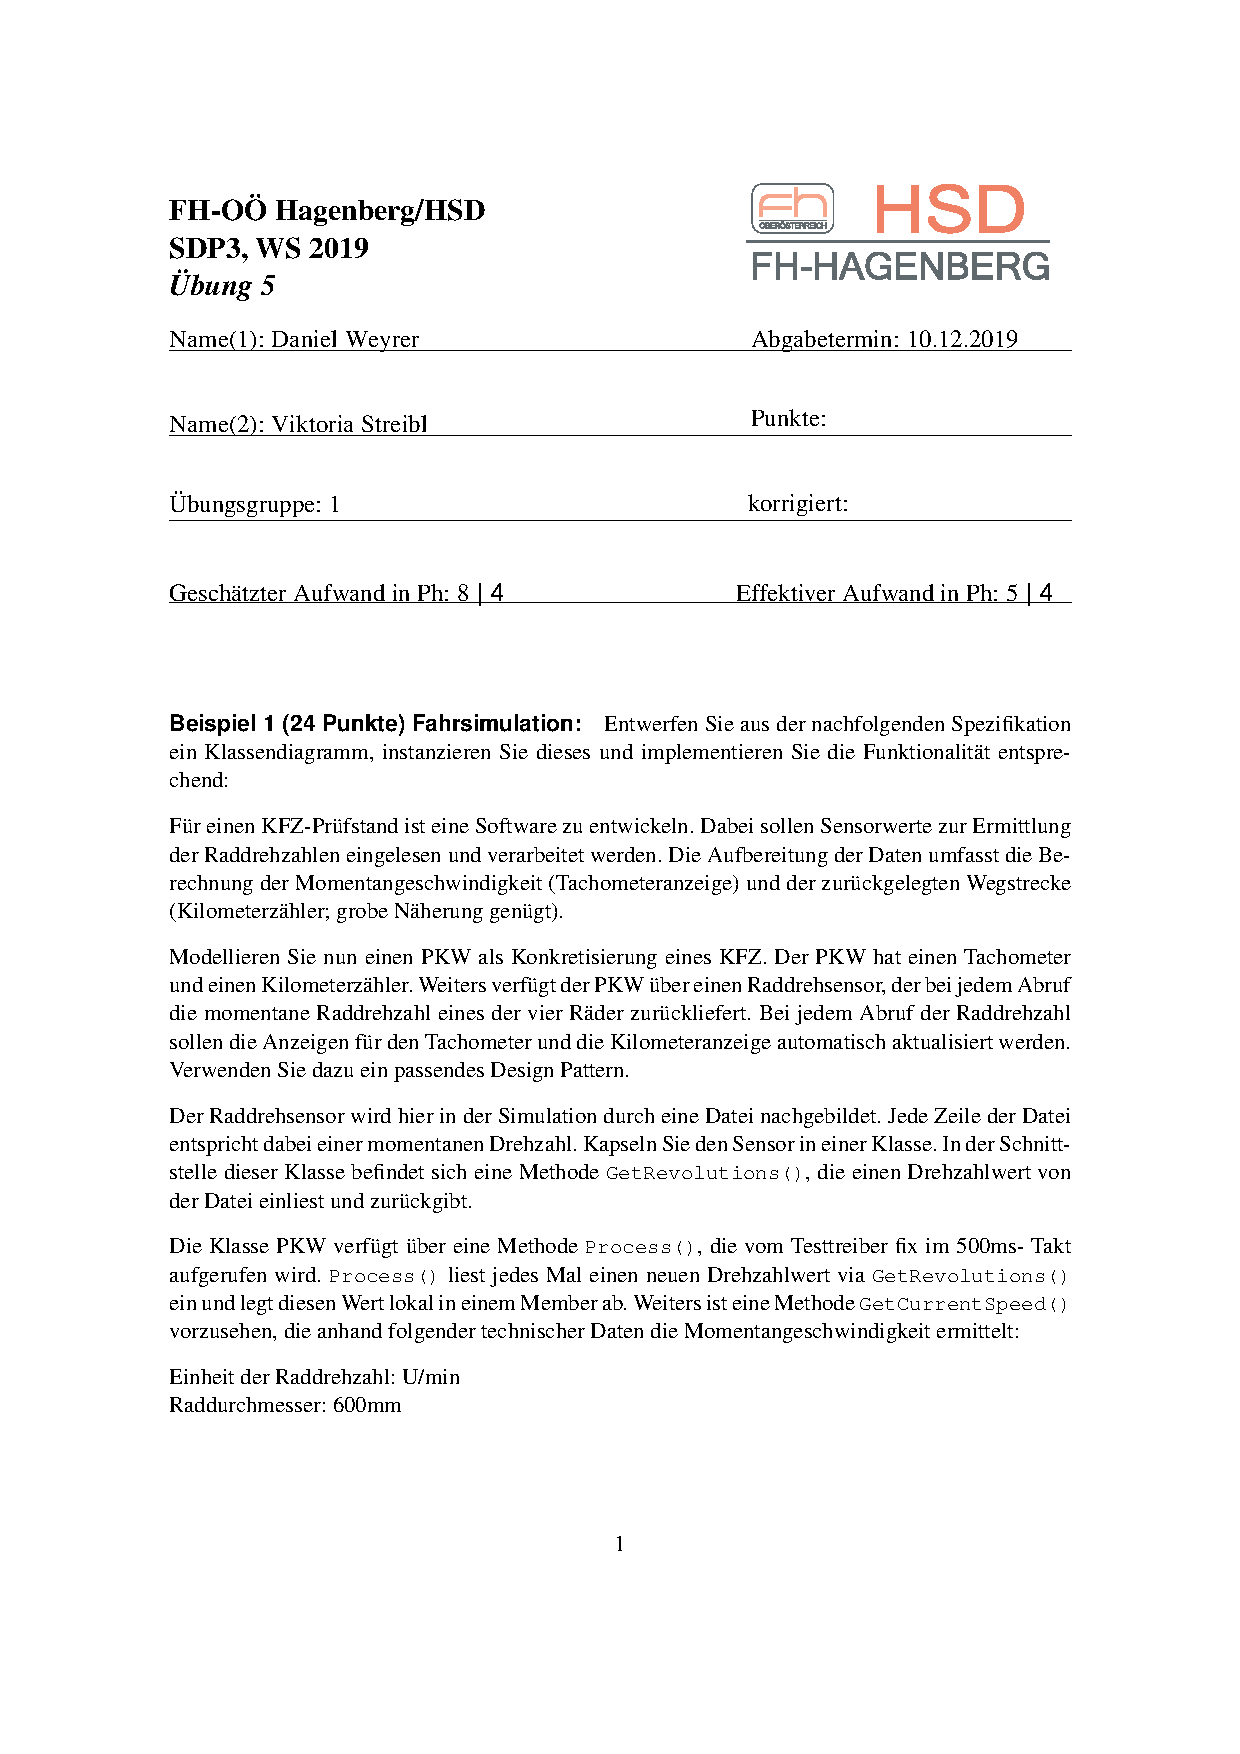
\includepdf[pages=-]{Angabe.pdf}

\title{SDP - Exercise 05} % Übungsname und Nummer angeben
\subtitle{winter semester 2019/20} % Semester angeben oder auskommentieren, falls nicht erwünscht
\author{
Viktoria Streibl - S1810306013\\
  Daniel Weyrer - S1820306044
} % Autorenname
\date{\today} % Das heutige Datum automatisch einfügen

\maketitle % Titelseite erstellen

\newpage
\tableofcontents % Inhaltsverzeichnis erstellen
\newpage

\ihead{Viktoria Streibl}
\ohead{Daniel Weyrer}
\chead{SDP3-UE Uebung 05}

\section{Organizational}
\subsection{Team}
\begin{itemize}
	\item Viktoria 	Streibl 		- 	S1810306013
	\item Daniel 	Weyrer		-	S1820306044
\end{itemize}

\subsection{Roles and responsibilities}
\subsubsection{Jointly}
\begin{itemize}
	\item Planning
	\item Documentation
	\item Systemdocumentation
	\item Class Diagram
\end{itemize}

\subsubsection{Viktoria Streibl}
\begin{itemize}
	\item Class IDisplay
	\subitem Class Speed
	\item Testdriver
\end{itemize}

\subsubsection{Daniel Weyrer}
\begin{itemize}
	\item Class Vehicle
		\subitem Class Car
		\subitem Class RPMSensor
	\item Class Distance
	
	
\end{itemize}

\subsection{Effort}

\subsubsection {Viktoria Streibl}
\begin{itemize}
	\item estimated: 6 ph 
	\item actually: 4 ph
\end{itemize}

\subsubsection {Daniel Weyrer}
\begin{itemize}
	\item estimated: 8 ph 
	\item actually: 5 ph
\end{itemize}


\section{System Design}
\subsection{Classdiagram}
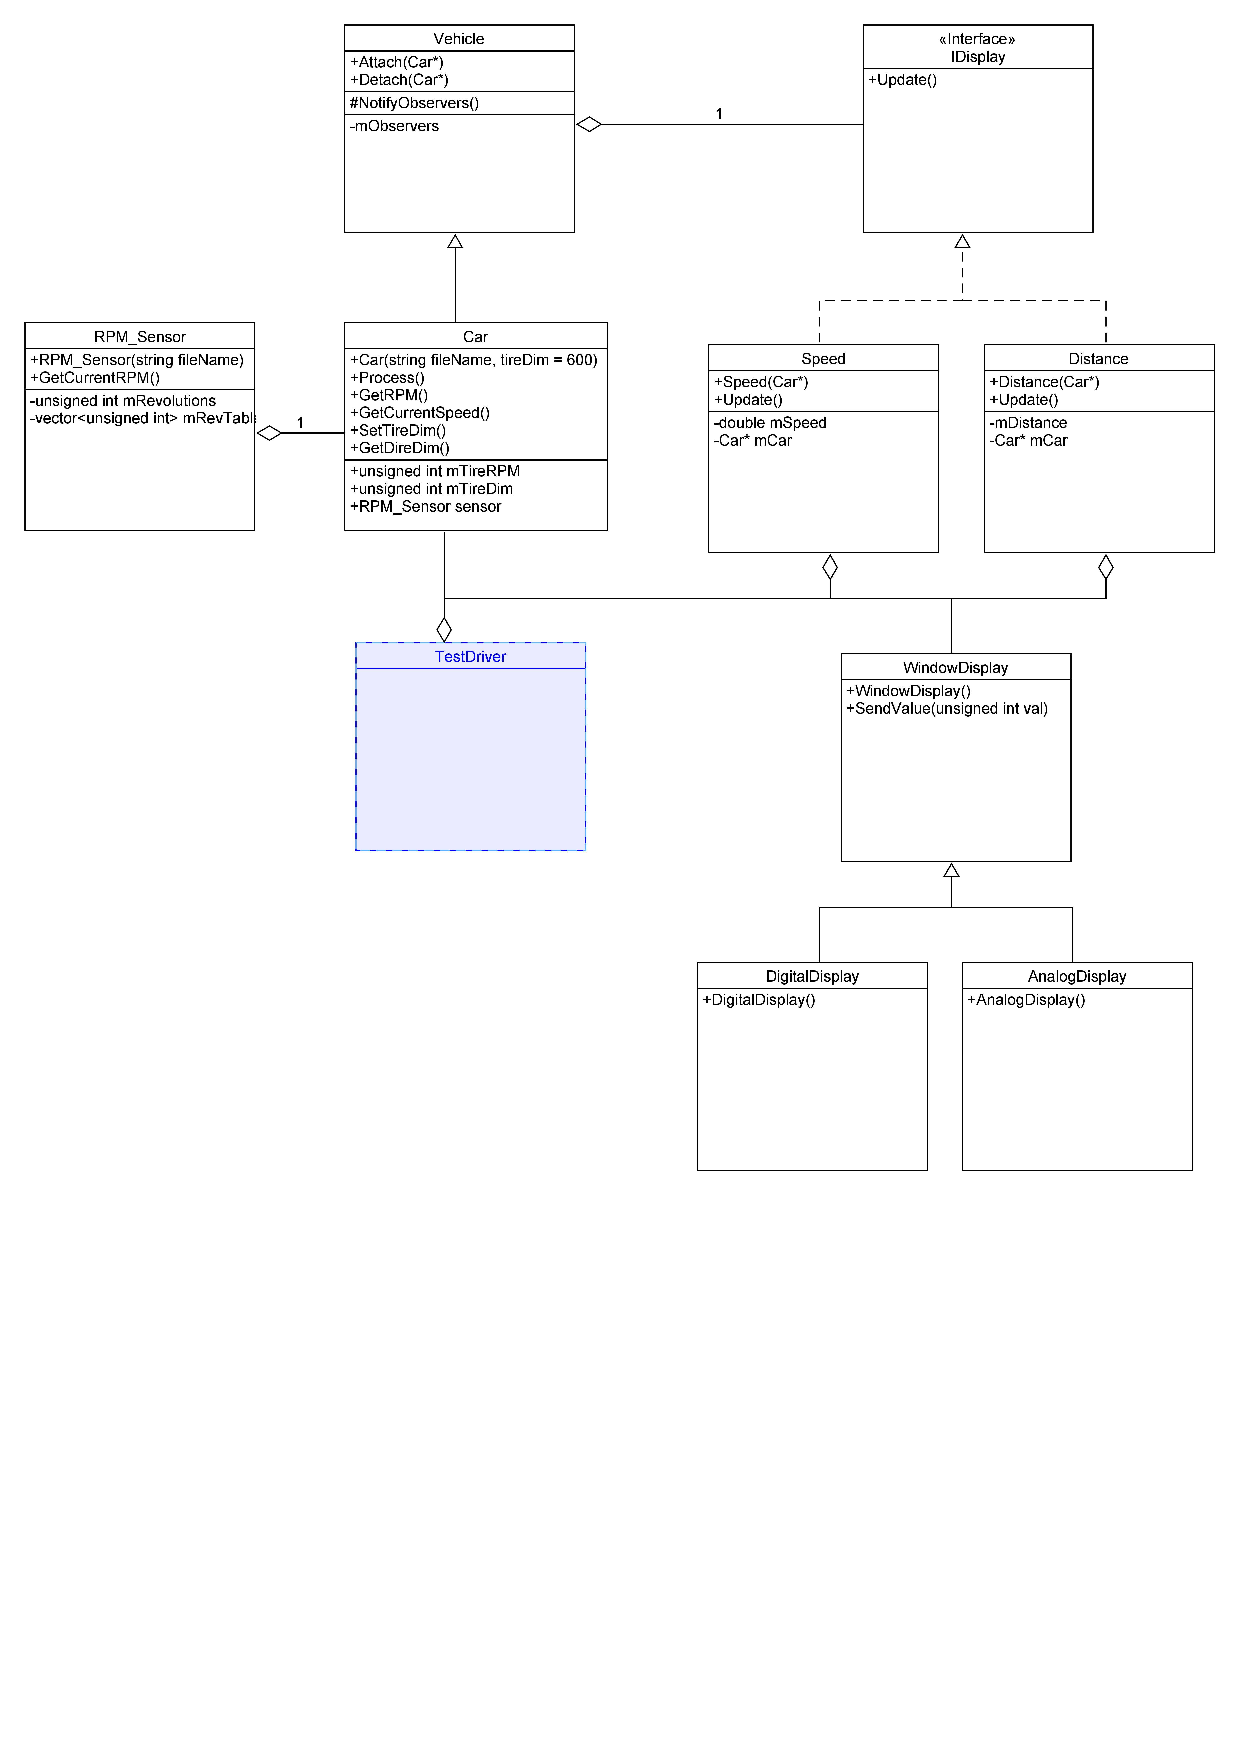
\includegraphics[scale=0.65]{ClassDiagramm1}

\subsection{Design Decisions}
\subsubsection{FileName in Constructor for Car}
As the Sensor is only simulated and useless without a fileName, we decided to store the fileName in the car class.

\subsubsection{ReadFile}
ReadFile uses the static filename given in the header to read the content to the container.


\newpage
\section{Test Protocol}

\subsection{Testfiles}
\subsubsection{output.txt}
\sourceCode{./DrivingSimulation/DrivingSimulation/output.txt}

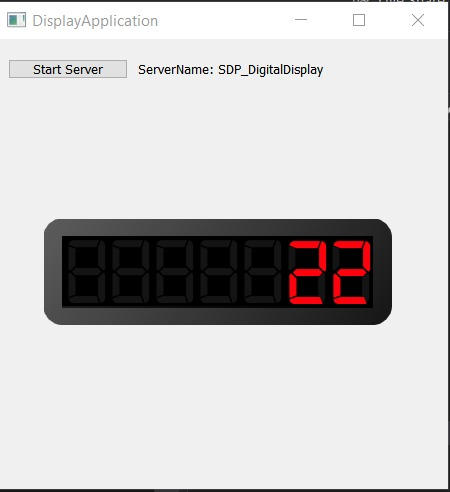
\includegraphics[scale=0.55]{DigitalDisplay.jpeg}
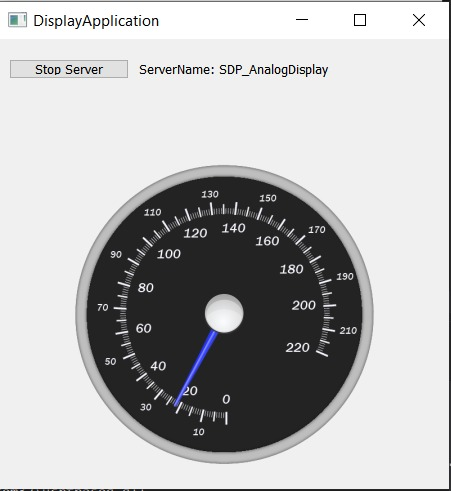
\includegraphics[scale=0.55]{AnalogDisplay.jpeg}

\newpage
\section{Source Code}

\subsection{Object.h}
\subsubsection{header.h}
\sourceCode{./DrivingSimulation/DrivingSimulation/Object.h}
\newpage


\subsection{Vehicle}
\subsubsection{Vehicle.h}
\sourceCode{./DrivingSimulation/DrivingSimulation/Vehicle.h}
\subsubsection{Vehicle.cpp}
\sourceCode{./DrivingSimulation/DrivingSimulation/Vehicle.cpp}
\newpage

\subsection{Car}
\subsubsection{Car.h}
\sourceCode{./DrivingSimulation/DrivingSimulation/Car.h}
\subsubsection{Car.cpp}
\sourceCode{./DrivingSimulation/DrivingSimulation/Car.cpp}
\newpage

\subsection{RPMSensor}
\subsubsection{RPMSensor.h}
\sourceCode{./DrivingSimulation/DrivingSimulation/RPMSensor.h}
\subsubsection{RPMSensor.cpp}
\sourceCode{./DrivingSimulation/DrivingSimulation/RPMSensor.cpp}
\newpage

\subsection{IDisplay}
\subsubsection{IDisplay.h}
\sourceCode{./DrivingSimulation/DrivingSimulation/IDisplay.h}
\newpage

\subsection{Speed}
\subsubsection{Speed.h}
\sourceCode{./DrivingSimulation/DrivingSimulation/Speed.h}
\subsubsection{Speed.cpp}
\sourceCode{./DrivingSimulation/DrivingSimulation/Speed.cpp}
\newpage

\subsection{Distance}
\subsubsection{Distance.h}
\sourceCode{./DrivingSimulation/DrivingSimulation/Distance.h}
\subsubsection{Distance.cpp}
\sourceCode{./DrivingSimulation/DrivingSimulation/Distance.cpp}
\newpage

\subsection{WindowsDisplay}
\subsubsection{WindowsDisplay.h}
\sourceCode{./DrivingSimulation/DrivingSimulation/WindowsDisplay.h}
\subsubsection{WindowsDisplay.cpp}
\sourceCode{./DrivingSimulation/DrivingSimulation/WindowsDisplay.h}


\subsection{TestDriver}
\subsubsection{TestDriver.cpp}
\sourceCode{./DrivingSimulation/DrivingSimulation/TestDriver.cpp}

% Um Quellcode einzufügen einfach diesen Befehl verwenden:
%\sourceCode{Relativer/Pfad/zum/SourceCode.Endung}

\section{Methoddescriptions}
\includepdf[pages=7-15]{refman.pdf}


\end{document}